\documentclass[twocolumn]{article}

\usepackage{float}
\usepackage{amsmath}
\usepackage{amsfonts}
\usepackage{textcomp}
\usepackage{gensymb}
\usepackage{amssymb}
\usepackage{tikz}

\begin{document}
\title{AP Physics C: Non-Conservative Forces Lab}
\author{Raja Williams}
\date{December 2023}

\twocolumn[
    \begin{@twocolumnfalse}
        \maketitle
        \begin{abstract}
            The purpose of this lab is to determine the coefficient of friction
            utilizing the energy lost in a half-Atwood system. Utilizing the
            difference between an ideal frictionless prediction of the kinetic
            energy and the kinetic energy based off of measurements one can find
            the loss from other forces, such as friction. To calculate the
            kinetic energy, we use derivations completed in class, which require
            $v$, which we measure through the Vernier Go
            Direct\textsuperscript{\tiny\textregistered} Sensor Cart. I am too
            lazy to actually learn the \texttt{titling} package to create a
            smaller abstract so I have just compensated by writing gibberish in
            the very large abstract at the top of the page.
        \end{abstract}
    \end{@twocolumnfalse}
]

\section{Procedure}
\begin{enumerate}
    \item
        Weigh the cart.
    \item
        Set up half-Atwood system as show in Figure \ref{fig:atwood}.

        \begin{figure}[h]
            \centering
            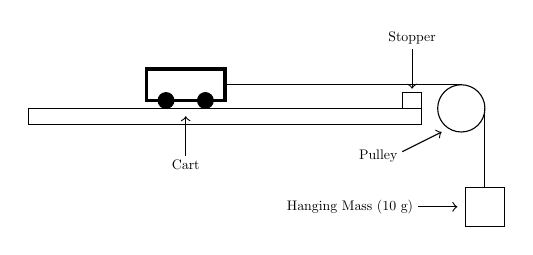
\begin{tikzpicture}[scale=0.5,transform shape]
                \draw[very thick] (0,0.2) rectangle (-2,1);
                \draw[fill=black] (-1.5,0.2) circle [radius=0.2];
                \draw[fill=black] (-0.5,0.2) circle [radius=0.2];
                \draw (6,0) circle [radius=0.6];
                \draw (0,0.6) -- (6,0.6);
                \draw (6.6,0) -- (6.6,-2);
                \draw (6.1,-2) rectangle (7.1,-3);
                \draw (4.5,0) rectangle (5,0.4);
                \draw (-5,0) rectangle (5,-0.4);
                \draw[->] (-1,-1.2) -- (-1,-0.2);
                \draw (-1,-1.2) node[anchor=north] {Cart};
                \draw[->] (4.5,-1.1) -- (5.5,-0.6);
                \draw (4.5,-1.2) node[anchor=east] {Pulley};
                \draw[->] (4.9,-2.5) -- (5.9,-2.5);
                \draw (4.9,-2.5) node[anchor=east] {Hanging Mass (10 g)};
                \draw[->] (4.75,1.5) -- (4.75,0.5);
                \draw (4.75,1.5) node[anchor=south] {Stopper};
            \end{tikzpicture}
            \caption{Diagram of half-Atwood setup used.}
            \label{fig:atwood}
        \end{figure}
    \item \label{itm:start}
        Start the recording from Vernier Graphical Analysis.
    \item
        Release the cart from a distance of one (1) meter from the stopper.
    \item
        Wait until the cart hits the stopper at the end of the track, and then
        stop the recording.
    \item
        Record the maximum velocity before the collision with stopper. If the
        mass hits the floor, record the maximum velocity before the mass hits
        the floor (visible as a plateau on the graph).
    \item
        If the mass hits the floor, measure the distance that the cart travels
        before the hanging mass hits the floor once.
    \item
        Repeat from Step \ref{itm:start} five (5) times.
\end{enumerate}

\section{Observations and Data}
The cart weighed 284 grams. The hanging mass hit the floor after travelling
0.71 meters.

\begin{figure}[h]
    \centering
    \begin{tabular}{| l | l |}
        \hline
        Trial & v (m/s) \\ \hline
        1 & 0.643 \\
        2 & 0.643 \\
        3 & 0.654 \\
        4 & 0.652 \\
        5 & 0.646 \\
        \hline
    \end{tabular}
    \caption{Table of data collected for $\overline{v}$.}
    \label{fig:v_data}
\end{figure}

\section{Data and Error Analysis}
Using the distance that the cart travels before the mass hits the floor, we can
predict the energy that the cart has. The difference between the ideal energy
and the real energy will allow us to predict the amount of energy lost to
friction, as the only other force on the cart should be the friction from the
pulley and the friction of the cart. These can be combined later to predict the
coefficient of friction $\mu$.

\begin{align}
    U_g &= 0.010 \text{ kg} \cdot 9.8 \text{ m/s\textsuperscript{2}} \cdot 0.71
        \text{ m} \\
    U_g &= 0.0696 \text{ J}
\end{align}

With the average velocity, we can find the actual kinetic energy that the cart
had before the mass hit the floor. Using the data in Figure \ref{fig:v_data}:

\begin{align}
    \overline{v} &= 0.646 \text{ m/s} \\
    KE &= \frac{1}{2} \cdot (0.284 \text{ kg} + 0.10 \text{ kg}) \cdot (0.646 \text{ m/s})^2 \\
    KE &= 0.0613 \text{ J}
\end{align}

Now the energy lost from the system from the friction force:

\begin{align}
    E_f &= 0.0696 \text{ J} - 0.0613 \text{ J} \\
    E_f &= 0.0082 \text{ J} \\
    \%E &= \frac{0.0082 \text{ J}}{0.0696 \text{ J}} \cdot 100
    \\
    \%E &= 11.8346\%
\end{align}

This means that 0.0082 J of the total energy of the system was lost to friction,
or about 11.8\% of the total energy of the system.

With the energy lost to friction, we can find the force of friction that acted
on the cart over the track. To make this calculation simpler, we assumed that
the friction force does not change over the track. Since the cart traveled 0.71
m, we can use the work integration to find the force:

\begin{align}
    0.0082 \text{ J} &= \int_{0 \text{ m}}^{0.71} F_f \,dx \\
    0.0082 \text{ J} &= 0.71 \text{ m} \cdot F_f - 0 \text{ m} \cdot F_f \\
    \label{equ:f_f} 0.0116 \text{ N} &= F_f
\end{align}

Now, with the force of friction, we can solve for the coefficient of friction,
$\mu$:

\begin{align}
    F_f &= 0.284 \text{ kg} \cdot 9.8 \text{ m/s\textsuperscript{2}} \cdot \mu
        \\
    0.0116 \text{ J} &= 0.284 \text{ kg} \cdot 9.8 \text{
        m/s\textsuperscript{2}} \cdot \mu \\
    \label{equ:mu} 0.004167 &= \mu
\end{align}

This assumes that all friction from the pulley is negligible.

\section{Conclusion}
I believe that the friction force is not necessarily negligible, considering the
percentage of energy lost just to friction. 10\% of the system energy is more
than enough to affect past labs which assumed the cart to be fully frictionless.

For example, the Netwon's 3\textsuperscript{rd} Law lab assumed that the cart
was frictionless. This could change the final result of the lab, making the
calculated $\mu$ far smaller than originally thought.

However, it could be argued that the $\mu$ that was calculated in Equation
\ref{equ:mu} is too small to affect measured velocity results, especially with
higher masses attached to the half-Atwood system. The force itself, calculated
in Equation \ref{equ:f_f}, only provides a counter-acceleration of about 0.041
m/s\textsuperscript{2} to the cart.

\end{document}
